% ColdRoute SG final report working draft.
% Import this file into Overleaf. Internal planning is in planning_notes.tex.
\documentclass[11pt,a4paper]{article}

\usepackage[margin=23mm]{geometry}
\usepackage[T1]{fontenc}
\usepackage{lmodern}
\usepackage{amsmath}
\usepackage{booktabs}
\usepackage{graphicx}
\usepackage{tikz}
\usetikzlibrary{arrows.meta}
\usepackage[hidelinks]{hyperref}

\newcommand{\TODO}[1]{\par\noindent\textbf{[TODO]}~#1\par}

\begin{document}



\begin{titlepage}
\centering
\vspace*{2.7cm}
{\Huge\bfseries ColdRoute SG\par}
\vspace{0.7cm}
{\Large Weather-, Traffic- and Parking-Aware\\
Cold-Chain Delivery Optimisation\par}
\vspace{1.3cm}
{\large CS5224 Cloud Computing --- Group Project\\Final Report (Working Draft)\par}
\vspace{1.6cm}
{\large\bfseries Group 36\par}
\vspace{0.55cm}
\begin{tabular}{ll}
\toprule
\textbf{Full name} & \textbf{NUS NetID} \\
\midrule
Kim Jae Hyeok & E0893439 \\
Agarwal Ishan & E1186264 \\
Ler Lian Ping & E1554646 \\
Chao Chien Hung & E1539132 \\
Passion Goh Wei Ling & E0560272 \\
Huang Xuan Kun & E0319118 \\
\bottomrule
\end{tabular}
\vfill
{\small Draft dated 14 October 2026. Findings and assignments remain to be verified.\par}
\end{titlepage}
\pagenumbering{arabic}

\begin{abstract}
ColdRoute SG is a prototype decision aid for a Singapore dispatcher planning one cold-chain delivery vehicle with 5--15 stops. It compares a shortest-travel-time route with a sequence that also considers delivery windows, short-term rain, parking difficulty and cargo sensitivity. This report describes the data joins, scoring method and cloud design, then evaluates route quality, usability and hosting cost. The proposed weights, price and market estimates in this working draft are hypotheses; measured results will be added after experiments.
\TODO{Replace the final sentence with measured headline results and limitations before submission.}
\end{abstract}

\section{Motivation and Business Case}
Last-mile cold-chain deliveries are sensitive to delays at both the road and the unloading point. A route that minimises driving time can still miss a delivery window or expose chilled goods to a longer wait. Our target user is a dispatcher at a small Singapore food or healthcare delivery operation. The prototype plans one known delivery run from one depot to 5--15 stops; it does not provide turn-by-turn navigation or measure cargo temperature.

Existing products already address much of the routing problem. OptimoRoute supports delivery time windows, driver workflows and route history, with a published Lite price of \$35.10 per driver per month when billed annually~\cite{optimoroute}. Onfleet offers route optimisation, a driver app and proof of delivery; its published Launch plan starts at \$619 per month for 2,500 tasks~\cite{onfleet}. These prices use the vendors' displayed \$ currency and different billing units, so they are not directly comparable to our proposed Singapore-dollar price. We do not assume that these products cannot support weather or cold-chain integrations. ColdRoute instead tests whether a focused, explainable planning view that uses local short-term weather and parking context is useful to this narrower user group.
\TODO{Add a compact side-by-side feature comparison and verify competitor pricing/currency at final submission. State the exact ColdRoute feature that a user study will test.}

\section{Business Model and Market Estimate}
The course prototype is free for demonstration. A possible commercial planning tier is \textbf{S\$49 per active vehicle per month}; this is a \emph{pricing hypothesis}, not a launched offer or validated willingness to pay. Multi-vehicle planning, tracking, integrations and temperature telemetry would require further development. Interviews with dispatchers should test current planning costs, the value of avoiding lateness, and reactions to several price points before a commercial claim is made.

For a transparent first market estimate, Enterprise Singapore's 2020/21 annual report described about 5,300 logistics SMEs in the scope of its digitalisation plan~\cite{esg}. This is a broad and dated denominator, \emph{not} a count of Singapore cold-chain delivery companies. Applying assumed eligibility shares and fleet sizes gives the illustrative annual subscription opportunities below at 100\% adoption within each filtered group:

\begin{center}
\begin{tabular}{lrrr}
\toprule
Scenario & Eligible firms & Vehicles per firm & Annual opportunity \\
\midrule
Narrow: 2\% of 5,300 & 106 & 1 & S\$62,328 \\
Base: 5\% of 5,300 & 265 & 2 & S\$311,640 \\
Wide: 10\% of 5,300 & 530 & 3 & S\$934,920 \\
\bottomrule
\end{tabular}
\end{center}
Each value is `eligible firms $\times$ vehicles per firm $\times$ S\$49 $\times$ 12'. The percentages and vehicle counts are unverified assumptions, and these figures are \emph{not} revenue forecasts. We will refine the eligible share using operator interviews and a deduplicated list of firms with their own temperature-sensitive last-mile fleet. SFA's counts of licensed coldstores and food-processing premises can be a cross-check, but premises are not unique firms and must not simply be added to the logistics-SME count~\cite{sfa}.
\TODO{Validate the eligible-company count, fleet-size assumptions and willingness to pay; report interviews or clearly retain these as illustrative scenarios. Compare proposed revenue with actual service cost.}

\section{Architecture and Implementation}
\subsection{System and Cloud Architecture}
\begin{figure}[htbp]
\centering
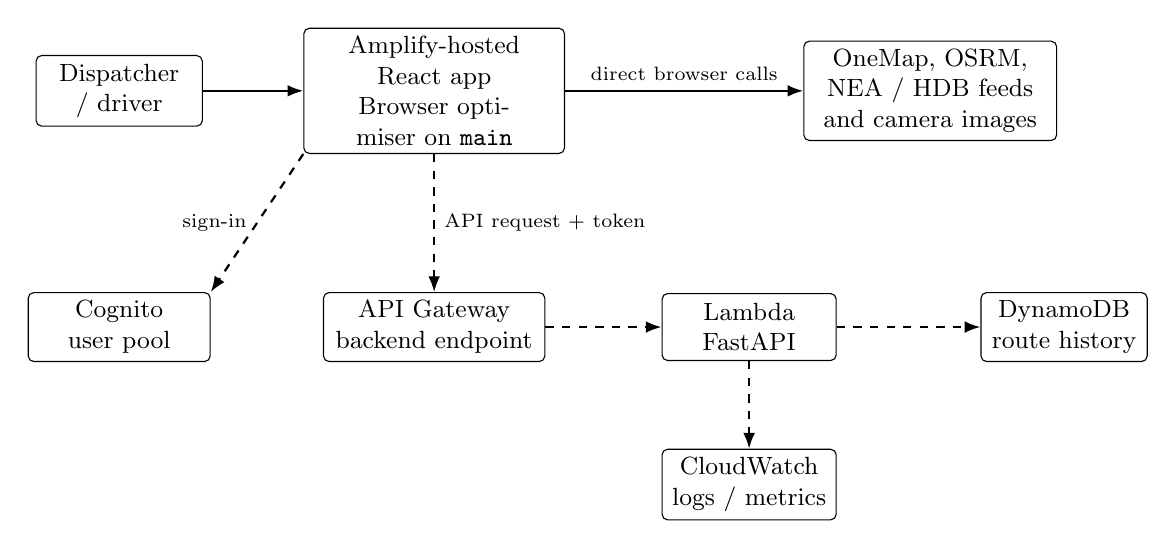
\begin{tikzpicture}[
  box/.style={draw, rounded corners=2pt, align=center, font=\small,
    minimum height=0.85cm, text width=2.6cm, inner sep=3pt},
  solidflow/.style={-{Latex[length=2mm]}, thick},
  plannedflow/.style={-{Latex[length=2mm]}, thick, dashed}
]
  \node[box, text width=1.9cm] (user) at (0,3) {Dispatcher / driver};
  \node[box, text width=3.1cm] (app) at (4,3) {Amplify-hosted React app\\Browser optimiser on \texttt{main}};
  \node[box, text width=3.0cm] (feeds) at (10.3,3) {OneMap, OSRM,\\NEA / HDB feeds\\and camera images};

  \node[box, text width=2.1cm] (cognito) at (0,0) {Cognito\\user pool};
  \node[box] (gateway) at (4,0) {API Gateway\\backend endpoint};
  \node[box, text width=2.0cm] (lambda) at (8,0) {Lambda\\FastAPI};
  \node[box, text width=1.9cm] (dynamo) at (12,0) {DynamoDB\\route history};
  \node[box, text width=2.0cm] (watch) at (8,-2) {CloudWatch\\logs / metrics};

  \draw[solidflow] (user) -- (app);
  \draw[solidflow] (app) -- node[above, font=\scriptsize] {direct browser calls} (feeds);
  \draw[plannedflow] (app.south west) -- node[left, font=\scriptsize] {sign-in} (cognito.north east);
  \draw[plannedflow] (app) -- node[right, font=\scriptsize] {API request + token} (gateway);
  \draw[plannedflow] (gateway) -- (lambda);
  \draw[plannedflow] (lambda) -- (dynamo);
  \draw[plannedflow] (lambda) -- (watch);
\end{tikzpicture}
\caption{Architecture status on 14 October 2026. Solid arrows show the deployed \texttt{main} frontend's currently documented flow. Dashed arrows show the AWS path reported by a team member and represented in an unmerged branch; end-to-end integration and access control still require verification.}
\label{fig:architecture}
\end{figure}

The current \texttt{main} branch serves a React dispatcher console through AWS Amplify. The browser obtains address matches from OneMap, drive-time and geometry estimates from OSRM, and public weather, carpark and camera feeds from data.gov.sg. It computes the route order in the browser and provides a recorded-data mode when live feeds cannot be used. A separate FastAPI backend exists locally but is not yet the planner used by this console.

On 14 October, a team member reported provisioning the cloud resources in this order: Lambda, API Gateway and its backend endpoint, Amplify frontend configuration, Cognito user pool and app client for drivers and administrators, DynamoDB, then CloudWatch monitoring. This is a \emph{reported deployment sequence}, not a verified end-to-end request trace. The intended runtime path is browser on Amplify $\rightarrow$ API Gateway $\rightarrow$ Lambda $\rightarrow$ DynamoDB, with Cognito issuing user tokens and CloudWatch collecting operational telemetry. The related code is present on an unmerged branch. Before describing this as the final implemented architecture, we must test a signed-in driver and admin against the actual API, confirm route ownership and persistence, inspect logs/metrics, and reconcile that branch with \texttt{main} without losing the existing console or CI.
\TODO{Verify the deployed API endpoint, Cognito sign-in for both roles, token enforcement, DynamoDB route ownership, CloudWatch metrics, and which branch is actually deployed. Update Figure~\ref{fig:architecture} to one final verified architecture.}

\subsection{Data Alignment and Provenance}
The planner needs all signals at the same decision point: a route run with a departure time, stop coordinates, service durations and delivery windows. OSRM provides travel times between stop coordinates. The NEA two-hour forecast is area-level and time-bounded; the current frontend assigns each stop the nearest named forecast area and checks whether predicted service overlaps rain in that forecast interval~\cite{nea}. HDB availability is reported by carpark ID; the frontend joins it to stored carpark coordinates and uses a reporting carpark only when it lies within 600\,m of a stop~\cite{hdb}. Free-space ratio and walking distance produce a parking-risk proxy. An HDB car space is not evidence that a delivery van has a usable loading bay.

LTA traffic cameras are displayed for context but their images are not converted to speed estimates. The current traffic-risk field is a sample or location-based proxy. LTA DataMall publishes directed road-segment speed bands at five-minute intervals~\cite{lta}; joining these to OSRM road legs would require access and map matching that have not yet been implemented. Until then, this report will distinguish OSRM travel estimates from measured live traffic. Each final experiment should store feed timestamps, validity windows and whether a value came from live, recorded or fallback data. Out-of-horizon weather and unavailable parking should be labelled unknown rather than silently assumed safe.
\TODO{Decide whether live LTA speed bands can be integrated. Document the exact spatial join, freshness threshold, and missing-data behaviour used in the final build; make the text match tested code.}

\subsection{Route Objective and Search}
The following is a \emph{proposed normalised objective for the final implementation}, not a description of the current code. For $n$ stops, let $T$ be total drive minutes, $L$ total late minutes, $W$ the sum of rain severity (0, 0.5 or 1) times service minutes, $P$ the sum of a 0--1 parking proxy times service minutes, and $C$ the sum of cargo sensitivity times minutes on board before service. These are operational proxies; $C$ is not a temperature or spoilage measurement.
\begin{equation}
J(r)=\alpha\widehat{T}(r)+\beta\widehat{L}(r)+
\gamma\widehat{W}(r)+\delta\widehat{P}(r)+\varepsilon\widehat{C}(r).
\end{equation}
For the first pilot, use fixed, per-stop reference scales:
\begin{equation}
\widehat{T}=\frac{T}{20n},\quad
\widehat{L}=\frac{L}{15n},\quad
\widehat{W}=\frac{W}{15n},\quad
\widehat{P}=\frac{P}{15n},\quad
\widehat{C}=\frac{C}{120n}.
\end{equation}
These denominators are \emph{initial assumptions} in minutes, not fitted results. We will inspect pilot-scenario distributions, freeze any revised scales before held-out evaluation, and report the chosen values. We do not rescale terms separately for each candidate route or cap severe lateness, which would make comparisons misleading.

An initial \emph{Balanced} weight hypothesis is $(\alpha,\beta,\gamma,\delta,\varepsilon)=(0.30,0.30,0.10,0.10,0.20)$: drive time and lateness each receive 30\%, weather and parking 10\% each, and cargo exposure 20\%. The weights are non-negative and sum to one. We will test trade-offs with operators, tune only on training scenarios, then run a sensitivity analysis with each non-travel weight varied by $\pm25\%$ and renormalised. Raw outcomes---lateness, travel time and exposure---must be reported alongside $J$.

The current frontend instead uses minute-equivalent penalties and preset profile coefficients; it exhaustively searches up to eight stops and uses 2-opt above eight. The local backend uses a different greedy score. Before claiming this normalised method as implemented, the team must adopt one canonical optimiser and update the code and evaluation fixtures accordingly. The comparison baseline is the sequence that minimises driving time under the same travel-time matrix.
\TODO{Choose and implement one canonical objective; justify/freeze reference scales and weights before held-out tests. Check that weather and parking effects are not counted twice.}

\section{Evaluation}
\subsection{System Quality and Performance}
\textbf{Proposed evaluation plan.} Freeze at least 24 scenarios before measuring: 5, 10 and 15 stops crossed with rain, parking shortage, tight time windows and high-priority cargo at two severity levels. Compare ColdRoute with the shortest-drive baseline on the same saved data snapshot. Record travel and late minutes, late-stop count, weather/parking exposure, cargo-exposure proxy, objective value and computation time. Remove one signal at a time to test whether it contributes as expected. A correct route must contain each stop exactly once and give reproducible results from the same snapshot. Candidate targets are a 10\% median improvement in the scenario's targeted raw risk metric, no more than 15\% median added drive time, and p95 planning time below three seconds for 15 stops on stated hardware. These are targets, not findings; failures will be reported.
\TODO{Freeze scenarios and acceptance criteria before running experiments. Add result tables/figures, sample sizes, device specification, data mode, variance and failed cases.}

\subsection{User Evaluation}
Recruit 8--12 users, including people familiar with delivery planning if possible. Ask them to create a run, identify the highest-risk stop, compare two routes, explain a changed stop order and rerun after changing a constraint. Record task completion, time, errors, explanation comprehension and a short usability score. Proposed thresholds are at least 80\% task completion and 80\% correct explanation comprehension. Participant background and any failures will be included so these small-sample results are not presented as market validation.
\TODO{Recruit participants, run the tasks, and report actual completion, errors, task time, explanation comprehension and usability responses.}

\subsection{Cloud and On-Premise Cost Comparison}
\TODO{Add measured AWS line items and an equivalent on-premise workload after the final architecture is deployed. Show cost per optimisation and monthly low/base/high volume, with free-tier credits disclosed separately. Do not invent a savings percentage.}

\section{Discussion, Limitations, and Future Work}
\TODO{Interpret trade-offs and failures. Distinguish cold-chain exposure proxy from measured temperature/spoilage, and camera images from traffic speeds. Separate implemented features from future work.}

\section{Code Explanation and Reproducibility}
\TODO{Give the public repository URL, key directories, build/run instructions, deployed demo URL, data-source dependencies, and how to reproduce evaluation runs. Check that the URL remains accessible until marks and feedback are released.}

\section*{AI Use Declaration and References}
\TODO{Declare where AI assisted with research, drafting, implementation or review, what was verified by the team, and what was learned, following course rules.}

\begin{thebibliography}{9}
\bibitem{course} CS5224, ``Group Project Specification,'' 2026.
\bibitem{optimoroute} OptimoRoute, ``Pricing,'' \url{https://optimoroute.com/pricing/}, accessed 14 October 2026.
\bibitem{onfleet} Onfleet, ``Pricing,'' \url{https://onfleet.com/pricing}, accessed 14 October 2026.
\bibitem{esg} Enterprise Singapore, ``Annual Report 2020--2021,'' \url{https://www.enterprisesg.gov.sg/-/media/esg/files/resources/publications/annual-reports/esg_ar2020_21.pdf}.
\bibitem{sfa} Singapore Food Agency, ``Singapore Food Statistics 2025,'' \url{https://www.sfa.gov.sg/news-publications/newsroom/singapore-food-statistics-2025}.
\bibitem{nea} data.gov.sg, ``2-hour Weather Forecast,'' \url{https://api.data.gov.sg/v1/environment/2-hour-weather-forecast}.
\bibitem{hdb} data.gov.sg, ``Carpark Availability,'' \url{https://data.gov.sg/datasets/d_ca933a644e55d34fe21f28b8052fac63/view}.
\bibitem{lta} Land Transport Authority, ``LTA DataMall API User Guide,'' \S2.19, \url{https://datamall.lta.gov.sg/content/dam/datamall/datasets/LTA_DataMall_API_User_Guide.pdf}.
\end{thebibliography}



\end{document}
